\documentclass{article}

\usepackage{graphicx}
\usepackage{rotating}
\usepackage{amsmath}
\usepackage{fancyhdr}
\usepackage{listings}
\usepackage{xcolor}
\usepackage{color}
\usepackage{textcomp}
\usepackage{float}
\usepackage[sorting=none]{biblatex}
\usepackage[margin=1in]{geometry}
\usepackage[font={small,it}]{caption}
\usepackage{placeins}
\usepackage{xepersian}

%\DeclareMathOperator*{\btie}{\bowtie}
\addbibresource{bibliography.bib}
\settextfont[Scale=1.2]{B-NAZANIN.TTF}
\setlatintextfont[Scale=1]{Times New Roman}
\renewcommand{\baselinestretch}{1.5}
\pagestyle{fancy}
\fancyhf{}
\rhead{تکلیف چهارم درس شبکه‌های کامپیوتری 2}
\lhead{\thepage}
\rfoot{علیرضا ابره فروش}
\lfoot{9816603}
\renewcommand{\headrulewidth}{1pt}
\renewcommand{\footrulewidth}{1pt}
%%%%%%%%%%
\lstset
{
    language=[latex]tex,
    basicstyle=\ttfamily,
    commentstyle=\color{black},
    columns=fullflexible,
    keepspaces=true,
    upquote=true,
    showstringspaces=false,
    morestring=[s]\\\%,
    stringstyle=\color{black},
}
%%%%%%%%%%
%beginMatlab
\definecolor{mygreen}{RGB}{28,172,0} % color values Red, Green, Blue
\definecolor{mylilas}{RGB}{170,55,241}
%endMatlab
\begin{document}
%beginMatlab
\lstset{language=Matlab,%
    %basicstyle=\color{red},
    breaklines=true,%
    morekeywords={matlab2tikz},
    keywordstyle=\color{blue},%
    morekeywords=[2]{1}, keywordstyle=[2]{\color{black}},
    identifierstyle=\color{black},%
    stringstyle=\color{mylilas},
    commentstyle=\color{mygreen},%
    showstringspaces=false,%without this there will be a symbol in the places where there is a space
    numbers=left,%
    numberstyle={\tiny \color{black}},% size of the numbers
    numbersep=9pt, % this defines how far the numbers are from the text
    emph=[1]{for,end,break},emphstyle=[1]\color{red}, %some words to emphasise
    %emph=[2]{word1,word2}, emphstyle=[2]{style},    
}
%endMatlab
\begin{titlepage}
\begin{center}

\includegraphics[width=0.4\textwidth]{figures/IUT Logo.png}\\
        
\LARGE
\textbf{دانشگاه صنعتی اصفهان}\\
\textbf{دانشکده مهندسی برق و کامپیوتر}\\
        
\vfill
        
\huge
\textbf{عنوان: تکلیف چهارم درس ریزپردازنده}\\
        
\vfill
        
\LARGE
\textbf{نام و نام خانوادگی: علیرضا ابره فروش}\\
\textbf{شماره دانشجویی: 9816603}\\
\textbf{نیم\,سال تحصیلی: پاییز 1400}\\
\textbf{مدرّس: دکتر عارف کریمی افشار}\\
\end{center}
\end{titlepage}


%\tableofcontents
\newpage


\section{سوال 14}
\subsection{\lr{a}}
پروتکل \lr{eBGP}
\subsection{\lr{b}}
پروتکل \lr{iBGP}
\subsection{\lr{c}}
پروتکل \lr{eBGP}
\subsection{\lr{d}}
پروتکل \lr{iBGP}

\section{سوال 15}
\subsection{\lr{a}}
از آنجایی که این اینترفیس کم‌هزینه‌ترین مسیر از \lr{1d} به \lr{1c} را آغاز می‌کند، $I$ برابر است با $I_{1}$.
\subsection{\lr{b}}
هر دو مسیر طول \lr{AS\_PATH} یکسانی دارند اما $I_{2}$ مسیری را که نزدیک‌ترین \lr{NEXT-HOP} روتر دارد را آغاز می‌کند.
\subsection{\lr{c}}
$I_{1}$ مسیری که کوتاه‌ترین \lr{AS-PATH} دارد را آغاز می‌کند.
\section{سوال 17}
\begin{figure}[H]
    \centering
    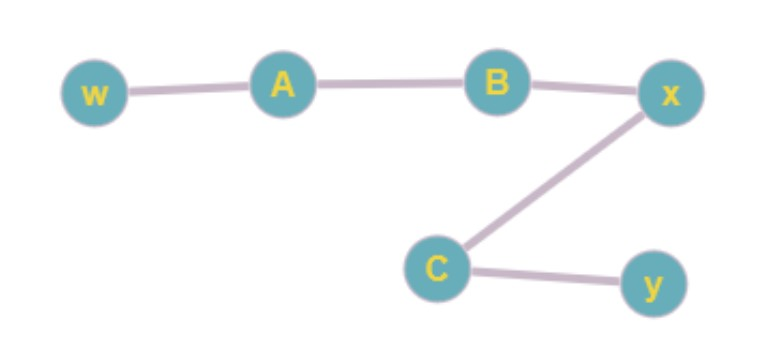
\includegraphics[width=1.0\textwidth]{figures/a.jpg}
    \caption
	{
نمای \lr{X} از توپولوژی
	}
    \label{fig:fig1}
\end{figure}
\begin{figure}[H]
    \centering
    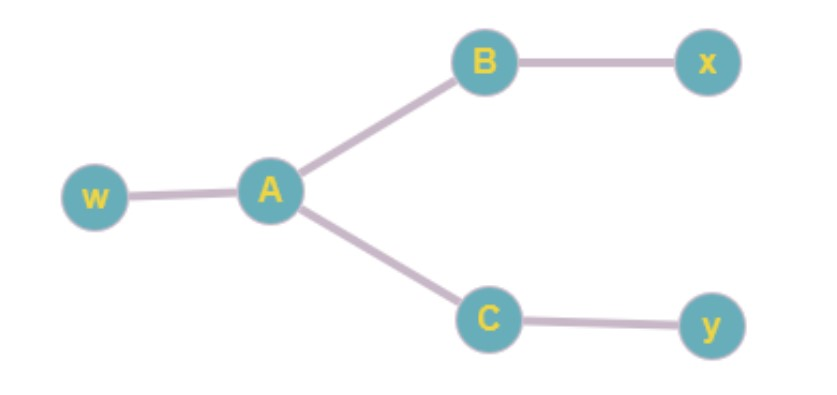
\includegraphics[width=1.0\textwidth]{figures/b.jpg}
    \caption
	{
نمای \lr{W} از توپولوژی
	}
    \label{fig:fig1}
\end{figure}
در این راه‌حل، از آنجایی که \lr{X} \lr{advertisement} مسیر به \lr{w} یا \lr{y} شامل لینک \lr{AC} را دریافت نکرده است، اطلاعی از لینک بین \lr{A} و \lr{C} ندارد. در واقع \lr{X} هیچ \lr{advertisement}ی شامل هر دوی \lr{AS A} و \lr{AS C} در مسیر مقصد ندارد.
\section{سوال 19}
\lr{A} باید 2 مسیرِ \lr{A-W} و \lr{A-V} را به \lr{B} پیشنهاد دهد.
\newline
\lr{A} باید تنها مسیرِ \lr{A-V} را به \lr{C} پیشنهاد دهد.
\newline
\lr{C} \lr{AS}مسیرهای \lr{B-A-W}، \lr{B-A-V} و \lr{A-V} را دریافت می‌کند.
\section{سوال 20}
از آنجایی که \lr{Z} می‌خواهد ترافیک \lr{Y} را انتقال دهد، مسیر را برای \lr{Y} \lr{advertize} می‌کند. در این رابطه وقتی که \lr{Y} دیتاگرامی به مقصدِ آی‌پی‌ای که قابلیت دسترسی با استفاده از \lr{Z} دارد را دارد، \lr{Y} می‌تواند دیتاگرام را توسط \lr{Z} بفرستد. هرچند اگر \lr{Z} مسیرها را برای \lr{Y} \lr{advertize} کند، \lr{Y} می‌تواند آن مسیرها را برای \lr{X} \lr{re-advertize} کند. در نتیجه، در این مورد، \lr{Z} هیچ کاری نمی‌تواند بکند تا جلوی انتقال ترافیک از \lr{X} توسط \lr{Z} را بگیرد.

%%%%%%%%%%%%%%%%%%%%%%%%%%%%%%%%%%%
%%%%%%%%%%%%%%%%%%%%%%%%%%%%%%%%%%%
%%%%%%%%%%%%%%%%%%%%%%%%%%%%%%%%%%%

\section*{منابع}
\renewcommand{\section}[2]{}%
\begin{thebibliography}{99} % assumes less than 100 references
%چنانچه مرجع فارسی نیز داشته باشید باید دستور فوق را فعال کنید و مراجع فارسی خود را بعد از این دستور وارد کنید


\begin{LTRitems}

\resetlatinfont

\bibitem{b1}
\end{LTRitems}

\end{thebibliography}


\end{document}
